%--- Implementation
\begin{figure}[!ht]
    \centering
    \caption[\emph{Plan Cuadrante} and Changes in Police Performance]{\emph{Plan Cuadrante} and Changes in Police Performance}
    \label{fig:figure05}
    \label{fig:police_performance}
    \label{fig:effectiveness_es}
    \begin{subfigure}[t]{0.44\textwidth}
        \centering
        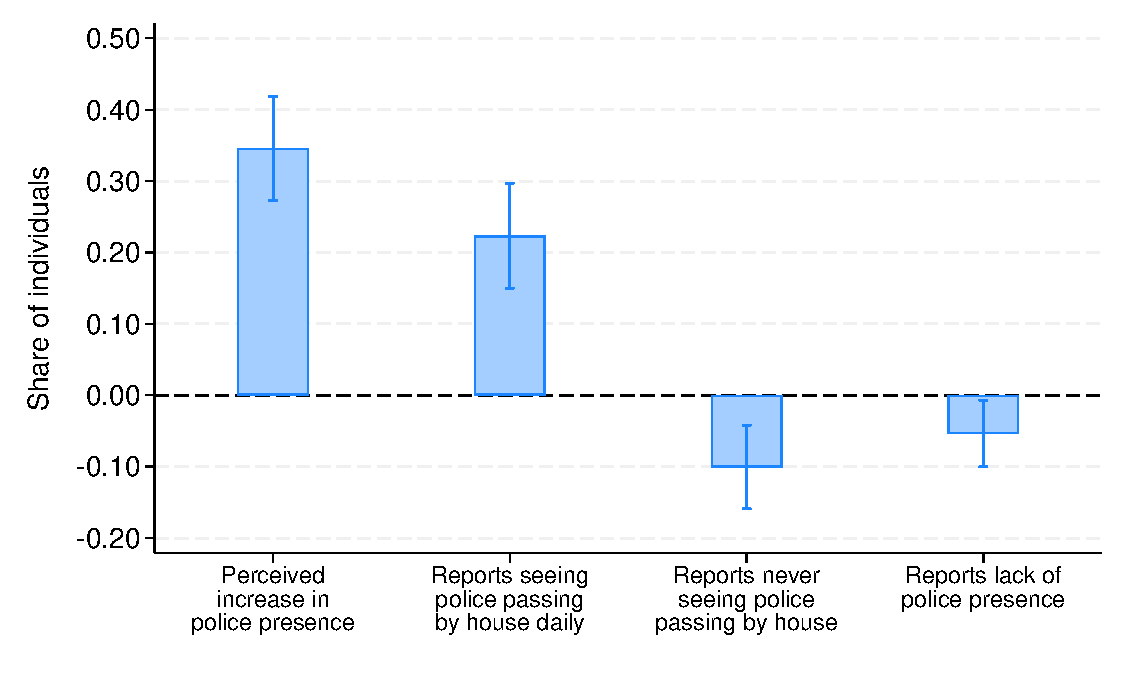
\includegraphics[width=\linewidth]{../manuscript/Graphs/results_policepresence.pdf}
        \caption{Effect on police presence}
    \end{subfigure}\hfill
    \begin{subfigure}[t]{0.44\textwidth}
        \centering
        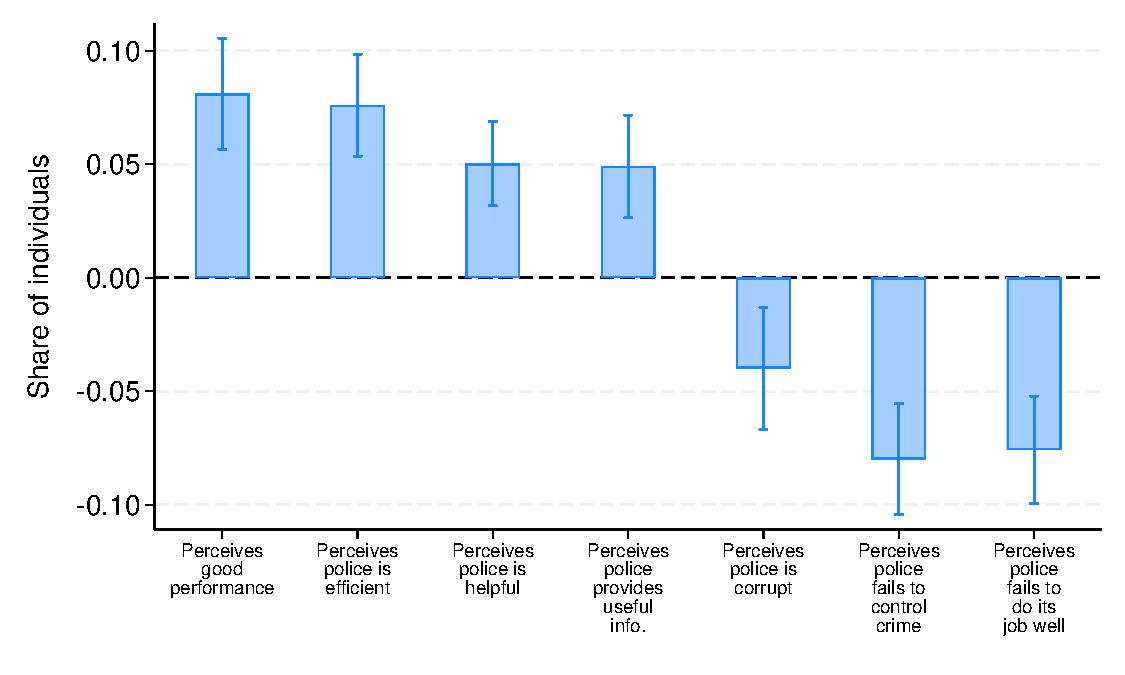
\includegraphics[width=\linewidth]{../manuscript/Graphs/combined_PCttest_2.pdf}
        \caption{Effect on perceived police performance}
    \end{subfigure}
    \\[6pt]
    \begin{subfigure}[t]{0.44\textwidth}
        \centering
        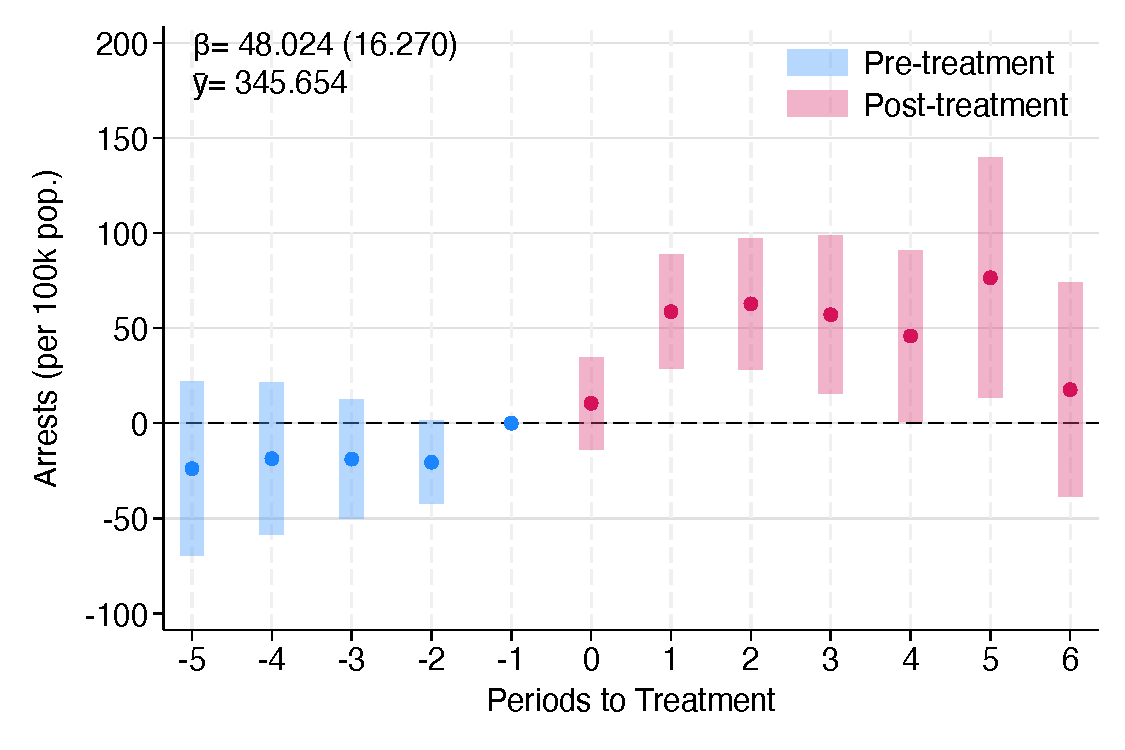
\includegraphics[width=\linewidth]{../manuscript/Graphs/totalarrestscrime_allcomunas.pdf}
        \caption{Arrests (per 100k pop.)}
    \end{subfigure}\hfill
    \begin{subfigure}[t]{0.44\textwidth}
        \centering
        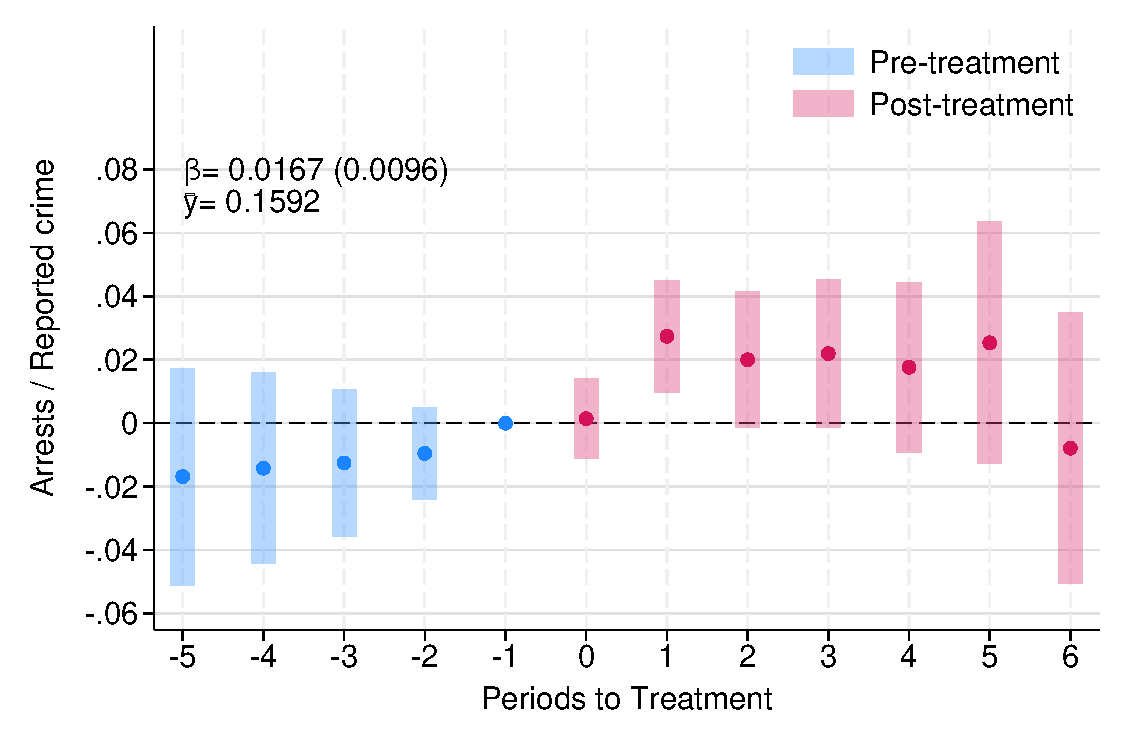
\includegraphics[width=\linewidth]{../manuscript/Graphs/arrests_over_reportedcrime_allcomunas.pdf}
        \caption{Arrests / Reported crime}
    \end{subfigure}
    \\[6pt]
    \begin{subfigure}[t]{0.44\textwidth}
        \centering
        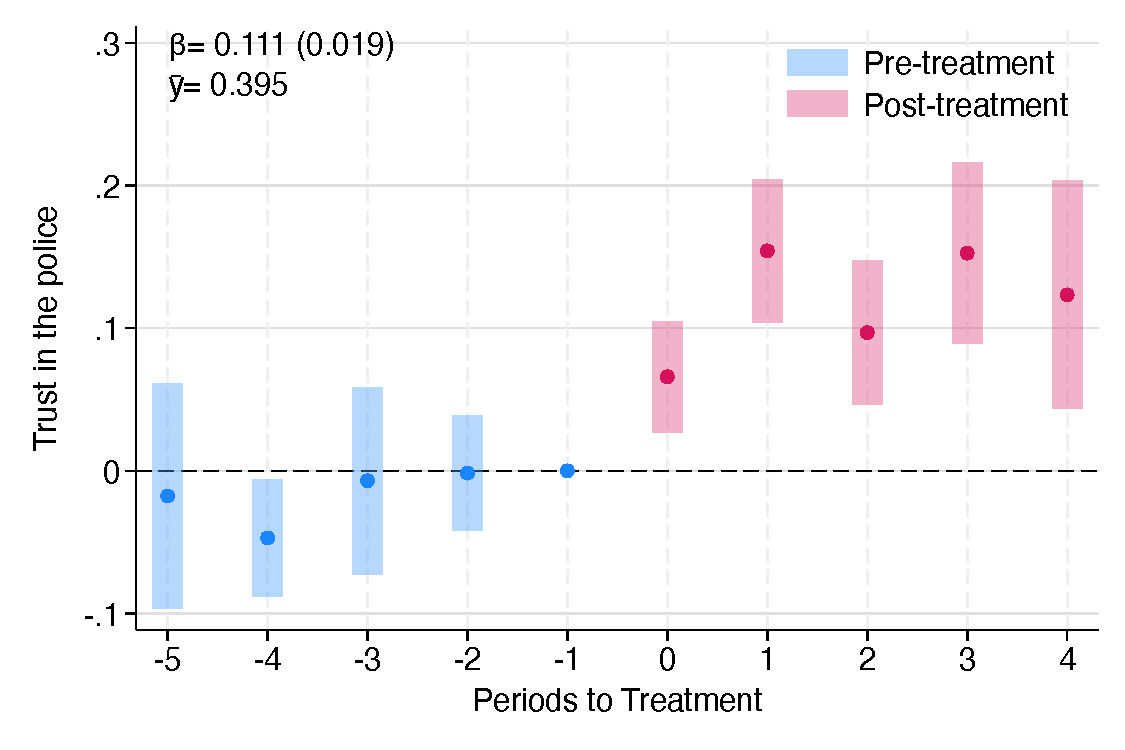
\includegraphics[width=\linewidth]{../manuscript/Graphs/results_trustcarabineros.pdf}
        \caption{Trust in the police}
    \end{subfigure}
    \\[8pt]
    \begin{minipage}{0.99\textwidth}
    \footnotesize Notes: Panel (a) reports the effects on perceived police presence. Panel (b) reports perceived police performance in 2005, comparing municipalities where \emph{Plan Cuadrante} was already implemented before 2006 with municipalities where it was implemented after 2005. Panels (c), (d), and (e) report dynamic event-study estimates for arrests per 100,000 inhabitants, the ratio of arrests to reported crime, and trust in the police. The estimation follows \citet{Callaway}. The graphs display estimated coefficients and 95\% confidence intervals. Standard errors are clustered at the municipality level using the wild bootstrapping procedure.
    \end{minipage}
\end{figure}
